% Sample article: firstarticle.tex, with index

\documentclass{amsart}
\usepackage{amssymb,latexsym}
\usepackage{graphicx}
\newtheorem{theorem}{Theorem}
\newtheorem{lemma}{Lemma}
\newtheorem{definition}{Definition}
\newtheorem{notation}{Notation}

\begin{document}
\title{A construction of complete-simple\\  
       distributive lattices}
\author{George~A. Menuhin}
\address{Computer Science Department\\
         University of Winnebago\\
         Winnebago, MN 53714} 
\date{March 15, 2006}

\begin{abstract}
   In this note, we prove that there exist 
   \emph{complete-simple distributive lattices,} 
   that is, complete distributive lattices
  with only two complete congruences. 
\end{abstract}

\maketitle

\section{Introduction}\label{S:intro} 
In this note, we prove the following result:

\begin{theorem} 
There exists an infinite complete distributive 
lattice~$K$ with only the two trivial complete 
congruence relations.
\end{theorem}

\section{The $\Pi^{*}$ construction}\label{S:P*} 
The following construction is crucial in the proof
of our Theorem (see Figure~\ref{Fi:products}):

\begin{definition}\label{D:P*} 
Let $D_{i}$, for $i \in I$, be complete distributive 
lattices satisfying condition~\textup{(J)}.  Their 
$\Pi^{*}$ product is defined as follows:
\[
   \Pi^{*} ( D_{i} \mid i \in I ) = 
   \Pi ( D_{i}^{-} \mid i \in I ) + 1;
\]
that is, $\Pi^{*} ( D_{i} \mid i \in I )$ is 
$\Pi ( D_{i}^{-} \mid i \in I )$ with a new 
unit element. 
\end{definition}

\begin{notation}
If $i \in I$ and $d \in D_{i}^{-}$, then
\[
  \langle \dots, 0, \dots, d, \dots, 0, \dots \rangle
\]
is the element of $\Pi^{*} ( D_{i} \mid i \in I )$ whose 
$i$-th component is $d$ and all the other components 
are $0$.
\end{notation}

See also Ernest~T. Moynahan~\cite{eM57a}.

Next we verify the following result:

\begin{theorem}\label{T:P*} 
Let $D_{i}$, $i \in I$, be complete distributive 
lattices satisfying condition~\textup{(J)}.  
Let $\Theta$ be a complete congruence relation on 
$\Pi^{*} ( D_{i} \mid i \in I )$. 
If there exist $i \in I$ and $d \in D_{i}$ with 
$d < 1_{i}$ such that, for all $d \leq c < 1_{i}$, 
\begin{equation}\label{E:cong1} 
   \langle \dots, d, \dots, 0, \dots \rangle \equiv 
   \langle \dots, c, \dots, 0, \dots \rangle 
   \pod{\Theta}, 
\end{equation}
then $\Theta = \iota$.
\end{theorem}

\begin{figure}[hbt]
\centering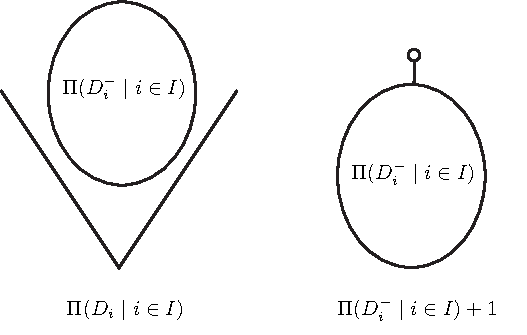
\includegraphics{products}
\caption{}\label{Fi:products}
\end{figure}

\begin{proof}
Since 
\begin{equation}\label{E:cong2}
\langle \dots, d, \dots, 0, \dots \rangle \equiv 
\langle \dots, c, \dots, 0, \dots \rangle 
\pod{\Theta}, 
\end{equation}
and $\Theta$ is a complete congruence relation, 
it follows from condition~(J) that
\begin{equation}\label{E:cong}
 \langle \dots, d, \dots, 0, \dots \rangle \equiv
 \bigvee ( \langle \dots, c, \dots, 0, \dots \rangle 
 \mid d \leq c < 1 ) \pod{\Theta}. 
\end{equation}

Let $j \in I$, $j \neq i$, and let $a \in D_{j}^{-}$. 
Meeting both sides of the congruence \eqref{E:cong2} 
with $\langle \dots, a, \dots, 0, \dots \rangle$, 
we obtain that
\begin{equation}\label{E:comp}
   0 = \langle \dots, a, \dots, 0, \dots \rangle 
     \pod{\Theta}, 
\end{equation}
Using the completeness of $\Theta$ and \eqref{E:comp}, 
we get:
\[
   0 \equiv \bigvee ( \langle \dots, a, \dots, 0, 
     \dots \rangle \mid a \in D_{j}^{-} ) = 1 
     \pod{\Theta}, 
\]
hence $\Theta = \iota$.
\end{proof}

\begin{thebibliography}{9}

\bibitem{sF90}
Soo-Key Foo, 
\emph{Lattice Constructions}, 
Ph.D. thesis, 
University of Winnebago, Winnebago, MN, December, 1990.

\bibitem{gM68}
George~A. Menuhin, 
\emph{Universal algebra}.
D.~Van Nostrand, Princeton, 1968.

\bibitem{eM57}
Ernest~T. Moynahan, 
\emph{On a problem of M. Stone},
Acta Math. Acad. Sci. Hungar. \textbf{8} (1957), 
455--460.

\bibitem{eM57a}
Ernest~T. Moynahan, 
\emph{Ideals and congruence relations in lattices.} II,
Magyar Tud. Akad. Mat. Fiz. Oszt. K\"{o}zl. \textbf{9} 
(1957), 417--434.

\end{thebibliography}

\end{document}

